%----------------------------------------------------------------------------------------
%    PACKAGES AND THEMES
%----------------------------------------------------------------------------------------

\documentclass{beamer}
\usetheme{Madrid}

\usepackage{hyperref}
\usepackage{graphicx} % Allows including images
\usepackage{booktabs} % Allows the use of \toprule, \midrule and \bottomrule in tables
\usepackage{siunitx}  % For formatting units and numbers, e.g., solar mass symbol
\usepackage{amsmath}  % For mathematical equations
\usepackage{listings}
\usepackage{xcolor}
\lstset{
    mathescape=false,
    texcl=false
}


%----------------------------------------------------------------------------------------
%    TITLE PAGE
%----------------------------------------------------------------------------------------

\title[Mass Density Profiles]{Mass Density Profiles in Globular and Open Clusters}
\subtitle{A Comparative Study of M2 and M34}

\author{Chiara Caserta Lopez \& Nathan Madsen}

\institute
{
    Department of Physics, Physics 134 \\
    UC Santa Barbara
}
\date{\today}

%----------------------------------------------------------------------------------------
%    PRESENTATION SLIDES
%----------------------------------------------------------------------------------------

\begin{document}

\begin{frame}
    \titlepage
\end{frame}

\begin{frame}{Introduction to Star Clusters}
    \begin{itemize}
        \item Gravitationally bound groups of stars that formed from the same giant molecular cloud.
        \item Act as a natural laboratory for studying stellar evolution.
        \item Two main types: \alert{Open clusters} and \alert{Globular clusters}.
    \end{itemize}
\end{frame}

\begin{frame}{What is a Mass Density Profile?}
    \begin{itemize}
        \item A function that describes how the density of stars or mass changes with distance from a cluster's center.
        \item Provides insight into a cluster's internal structure and dynamical evolution.
    \end{itemize}
    \begin{figure}
        \centering
        % Placeholder for a general density profile graph
        \includegraphics[width=0.7\textwidth]{Plummer_rho.png}
        \caption{A stylized depiction of a mass density profile, showing density decreasing with radius.}
    \end{figure}
\end{frame}

\section{The Plummer Model}

\begin{frame}{The Plummer Model}
    \begin{itemize}
        \item Proposed 1911 as a mathematical model for globular clusters. \cite{p1}
        \item Provides a simple, analytically tractable representation of a spherical system, featuring a core of constant density that transitions to a steeper fall-off at larger radii.
        \item This model is particularly useful for studying the dynamics of clusters, as it offers a smooth, continuous description of the mass distribution.
    \end{itemize}
\end{frame}

\begin{frame}{Plummer Model: The Potential $\Phi(r)$}
    \begin{itemize}
        \item The model is defined by its gravitational potential, $\Phi(r)$, which is given by:
        $$ \Phi(r) = - \frac{GM}{\sqrt{r^2 + a^2}} $$
        where:
        \begin{itemize}
            \item $G$ is the gravitational constant.
            \item $M$ is the total mass of the cluster.
            \item $a$ is the Plummer radius, a scale parameter that sets the size of the cluster's core.
        \end{itemize}
        \item This potential approaches that of a point mass ($-\frac{GM}{r}$) for $r \gg a$.
    \end{itemize}
\end{frame}

\begin{frame}{Plummer Model: Deriving the Density $\rho(r)$}
    \begin{itemize}
        \item The relationship between potential $\Phi(r)$ and mass density $\rho(r)$ is given by Poisson's equation:
        $$ \nabla^2 \Phi = 4 \pi G \rho $$
        \item In spherical coordinates, Poisson's equation for a spherically symmetric system simplifies to:
        $$ \frac{1}{r^2} \frac{d}{dr} \left( r^2 \frac{d\Phi}{dr} \right) = 4 \pi G \rho(r) $$
    \end{itemize}
\end{frame}

\begin{frame}{Derivation Step 1: Radial Derivative}
    \begin{itemize}
        \item We begin by taking the first radial derivative of the potential $\Phi(r)$:
        $$ \Phi(r) = -GM(r^2 + a^2)^{-1/2} $$
        $$ \frac{d\Phi}{dr} = -GM \left( -\frac{1}{2} \right) (r^2 + a^2)^{-3/2} (2r) $$
        $$ \frac{d\Phi}{dr} = \frac{GMr}{(r^2 + a^2)^{3/2}} $$
    \end{itemize}
\end{frame}

\begin{frame}{Derivation Step 2: Second Radial Derivative}
    \begin{itemize}
        \item Next, we multiply by $r^2$ and take the derivative again:
        $$ r^2 \frac{d\Phi}{dr} = \frac{GMr^3}{(r^2 + a^2)^{3/2}} $$
        \item Now, differentiate this expression with respect to $r$:
        \begin{align*} \frac{d}{dr} \left( r^2 \frac{d\Phi}{dr} \right) &= GM \frac{d}{dr} \left( \frac{r^3}{(r^2 + a^2)^{3/2}} \right) \\ &= GM \left[ \frac{3r^2(r^2 + a^2)^{3/2} - r^3 \cdot \frac{3}{2}(r^2 + a^2)^{1/2}(2r)}{(r^2 + a^2)^3} \right] \\ &= GM \left[ \frac{3r^2(r^2 + a^2) - 3r^4}{(r^2 + a^2)^{5/2}} \right] \\ &= GM \left[ \frac{3r^4 + 3a^2r^2 - 3r^4}{(r^2 + a^2)^{5/2}} \right] \\ &= \frac{3GMa^2r^2}{(r^2 + a^2)^{5/2}} \end{align*}
    \end{itemize}
\end{frame}

\begin{frame}{Derivation Step 3: Solve for $\rho(r)$}
    \begin{itemize}
        \item Substitute the result back into Poisson's equation:
        $$ \frac{1}{r^2} \left( \frac{3GMa^2r^2}{(r^2 + a^2)^{5/2}} \right) = 4 \pi G \rho(r) $$
        \item Simplify and solve for $\rho(r)$:
        $$ \frac{3GMa^2}{(r^2 + a^2)^{5/2}} = 4 \pi G \rho(r) $$
        $$ \rho(r) = \frac{3M}{4\pi a^3} \frac{1}{\left(1 + \frac{r^2}{a^2}\right)^{5/2}} $$
    \end{itemize}
\end{frame}

\begin{frame}{Plummer Model: Key Features}
    \begin{itemize}
        \item \textbf{Central Core:} As $r \to 0$, the density approaches a constant value:
        $$ \rho(0) = \frac{3M}{4\pi a^3} $$
        \item \textbf{Outer Profile:} As $r \to \infty$, the density falls off steeply as $r^{-5}$:
        $$ \rho(r) \propto r^{-5} $$
    \end{itemize}
\end{frame}

\section{Signal to Noise Ratio}
\begin{frame}{S/N Formula}
    \begin{itemize}
        \item \textbf{Signal: }
        $$ S = F A_\epsilon \tau$$
        \item \textbf{Noise:}
        $$N_T^2 = N_R^2 + N_S^2 + N_{DC}^2 + N_\beta^2$$
        \item \textbf{Signal to Noise:}
        $$S/N = \frac{F A_\epsilon \tau}{\big( N_R^2 + \tau (F A_\epsilon + i_{DC} + F_\beta A_\epsilon \Omega)\big)^{1/2}}$$ \cite{p2}
    \end{itemize}
\end{frame}

\definecolor{backcolour}{rgb}{0.95,0.95,0.92}
\begin{frame}[fragile]{Implementation}
    \begin{lstlisting}[language=Python, 
                   basicstyle=\ttfamily\tiny,
                   keywordstyle=\color{blue},
                   stringstyle=\color{red},
                   backgroundcolor=\color{backcolour},
                   keywordstyle=\color{magenta},
                   commentstyle=\color{green!50!black},
                   showstringspaces=false,
                   numbers=left,
                   numsep=1pt,
                   numberstyle=\tiny\color{gray},
                   frame=single,
                   mathescape=false,
                   breaklines=true,
                   tabsize=2,
                   caption=S-N Calculation]
                   
target_flux = 3500 # photons/s/m^2 for Mag 16 star in M2
area_effective = 0.036
integration_time = 100
noise_readout = 1
dark_current = 0.0022
background_flux = 2.6*10**12 # photons/s/m^2/st
pixel_solid_angle = 1.28*10**-11 # steradians

def snr(target_flux, area_effective, integration_time,
        noise_readout, dark_current,
        background_flux, pixel_solid_angle):
    signal = target_flux * area_effective * integration_time
    noise_background = background_flux * area_effective * integration_time * pixel_solid_angle
    noise_dark = dark_current * integration_time
    source_noise = signal
    total_noise = (source_noise+noise_background+noise_dark+noise_readout**2)**0.5
    snr = signal / total_noise
    return snr
    \end{lstlisting}
\end{frame}

\begin{frame}{Multipixel S/N}
    \begin{figure}
        \centering
        \includegraphics[width=0.5\linewidth]{output.png}
        \caption{Multipixel S/N versus integration time}
    \end{figure}
\end{frame}

\section{Completeness Corrections}
\subsection{Theoretical Foundation}
\begin{frame}{Fundemental Problem}
    \begin{itemize}
        \item \textbf{Completeness:}
        $$C(m) := \frac{N_{detected}(m)}{N_{true}(m)}$$
        \item \textbf{Relation to LF:}
        $$\Phi_{obs}(m) = C(m) \cdot \Phi_{true}(m)$$
    \end{itemize}
\end{frame}

\begin{frame}{Sources of Incompleteness}
    \begin{itemize}
        \item Photon statistics
        \item Crowding
        \item Image quality
    \end{itemize}
\end{frame}

\begin{frame}{Mathematical Framework}
    $$P(m_{obs} | m_{true}) = \frac{1}{\sqrt{2\pi \sigma_m^2}} \exp\left[ -\frac{(m_{obs}-m_{true})^2}{2\sigma_m^2}\right]$$
    with $\sigma_m(m)$ as magnitude-dependent photometric uncertainty. So
    $$C(m_{true}) = \int_{-\infty}^{m_{lim}}P(m_{obs}|m_{true})dm_{obs}$$
    with $m_{lim}$ as limiting magnitude. So
    $$C(m) = \frac{1}{2} \left[ 1 + \mathrm{erf}\left( \frac{m_{50} - m}{\sqrt{2} \sigma_{comp}}\right)\right] $$
    with $m_{50}$ as $50\%$ completeness magnitude, $\sigma_{comp}$ controls steepness
\end{frame}

\begin{frame}{Position-Dependent Completeness}
    More realistically $C(m,\mathbf{r})$

    Radius dependent crowding
    $$C(m,\mathbf{r}) \approx C_0(m)\cdot f_{crowd}(\mathbf{r})$$
    Background varies
    $$C(m,x,y) \approx C_0(m) \cdot f_{bg}(x,y)$$
    example
    $$f_{crowd}(r) = \exp \left[ -\alpha \frac{\Sigma(r)}{\Sigma_0} \right]$$
\end{frame}

\subsection{Artificial Star Test}
\begin{frame}{Methodology}
    \begin{itemize}
        \item For a magnitude bin $m_i$ in $[m_{min}, m_{max}]$ generate $N_{add}$ stars with random positions $(x_i,y_i)$
        \item Use reduction pipeline
        \item Match recovered stars to input positions
        $$\Delta r_{ij} = \sqrt{(x_i-x_j^{rec})^2+(y_i-y_j^{rec})^2}$$
        \item say star recovered if
        $$\Delta r < r_{match}, \qquad |m_{rec}-m_{input}|<\Delta m_{max}$$
    \end{itemize}
\end{frame}
\begin{frame}{Calculating Completeness}
    Using recovered stars
    $$C(m_i) = \frac{N_{recovered}(m_i)}{N_{added}(m_i)}$$
    and uncertainty
    $$\sigma_C(m_i)=\sqrt{\frac{C(m_i)\big( 1 - C(m_i)\big)}{N_{added}(m_i)}}$$
    Repeat artificial star test $N_{MC}\approx 50-100$ times
    $$\sigma_C^{sys} = \mathrm{std}\big( \{ C_i(m)\}_{i=1}^{N_{MC}}$$
    total uncertainty
    $$\sigma_C^{total} = \sqrt{(\sigma_C^{stat})^2+(\sigma_C^{sys})^2}$$
\end{frame}
\begin{frame}{Fitting to Error Function Model}
    Using our set of completeness values $\{ C_i\pm \sigma_i\}$ at magnitudes $\{ m_i \}$ we fit and minimize
    $$\chi^2(\theta) = \sum_i \frac{[C_i-C(m_i; \theta)]^2}{\sigma_i^2}$$
    But least squares assumes errors are Gaussian (not true) and have constant variance (not true, depends on $N$). Instead, use binomial statistics. 
    $$N_{rec} \approx \mathrm{Binomial}(N_{add},C(m))$$
    or
    $$P(N_{rec}|N_{add}, C) = {N_{add} \choose N_{rec}}C^{N_{rec}}(1-C)^{N_{add}-N_{rec}} = \mathcal{L}(C|N_{rec},N_{add})$$
\end{frame}
\begin{frame}{Multiple Likelihood Bins}
    Say we test for magnitude bins $m_1, \dots , m_n$ and we want to fit $C(m;\theta)$. Assuming independence of bins
    $$\mathcal{L}(\theta|\mathrm{data}) = \prod_{i=1}^n {N_{add,i} \choose N_{rec,i}}C(m_i;\theta)^{N_{rec,i}}[1-C(m_i,\theta)]^{N_{add,i}-N_{rec,i}}$$
    or
    $$\ln \mathcal{L}(\theta) = \sum_{i=1}^n \{ N_{rec,i}\ln C(m_i;\theta)+[N_{add,i}-N_{rec,i}]\ln [1-C(m_i;\theta)]\}$$
    and
    $$\hat{\theta}_{MLE} = \arg \max_\theta \ln \mathcal{L}(\theta)$$
\end{frame}
\begin{frame}{Fisher Information Matrix}
    Then for errors. Define the Fisher information matrix $$ F_{jk} = - \left\langle \frac{\partial^2\ln \mathcal{L}}{\partial \theta_j \partial \theta_k} \right\rangle $$
    and the parameter covariance matrix 
    $$\mathrm{Cov}(\theta) = F^{-1}$$
    so $\sigma_{m_{50}} = \sqrt{[\mathrm{Cov}]_{11}}$ and $\sigma_{\sigma_{comp}} = \sqrt{[\mathrm{Cov}]_{22}}$
\end{frame}
\begin{frame}{Model Comparison}
    Compare different completeness functions (error function vs. hyperbolic tangent vs. Fermi-Dirac)
    $$\mathrm{AIC} = -2\ln \mathcal{L}_{max}+2k $$
    where $k$ is the number of parameters. 
\end{frame}
\begin{frame}{Goodness of Fit}
    The deviance measures how well our model fits:
    $$D = -2 \ln \mathcal{L}(\hat{\theta})$$
\end{frame}

\subsection{Richardson-Lucy Deconvolution}
\begin{frame}{Richardson-Lucy Deconvolution}
    \textbf{Problem}: We observe a distorted luminosity function
    $$\Phi_{obs}(m) = \int K(m,m')\Phi_{true}(m')dm' $$
    Where $K(m,m')$ is the kernel representing
    \begin{itemize}
        \item Completeness: stars at magnitude $m'$ might not be detected
        \item Photometric errors: star with true magnitude $m'$ measured as $m$
    \end{itemize}
    $$K(m,m')=C(m') \cdot P(m|m')$$
    assuming Gaussian photometric errors
    $$P(m|m') = \frac{1}{\sqrt{2\pi \sigma_m^2}}\exp \left[ - \frac{(m-m')^2}{2\sigma_m^2} \right] $$
\end{frame}
\begin{frame}{Richardson-Lucy Algorithm}
    We want to recover $\Phi_{true}$ from $\Phi_{obs}$. The naive approach is $\Phi_{true}=\Phi_{obs}/C(m)$. This ignores scattering. Instead be aim to maximize the likelihood under Poisson statistics and enforce positivity. Start with a guess $\Phi_{true}^{(0)} = \Phi_{obs}$ and iterate
    $$ \Phi_{true}^{(n+1)}(m') = \Phi_{true}^{(n)}(m')\int \frac{\Phi_{obs}(m)}{\left[ \int K(m,m'')\Phi_{true}^{(n)}(m'')dm''\right]}K(m,m')dm$$
\end{frame}

\section{Membership Determination}
\begin{frame}{The Fundemental Problem}
    We do not just observe stars in the cluster
    $N_{observed}(m,r,\mu,\text{color})=N_{cluster}+N_{foreground}+N_{background}$
    \textbf{Goal}: For each detected star $i$, assign a membership probability $P_{member,i}\in [0,1]$. Define
    $$\text{Purity} = \frac{N_{\text{true members classified as members}}}{N_{\text{all stars classified as members}}}$$
    $$\text{Completeness} = \frac{N_{\text{true members classified as members}}}{N_{\text{all true members}}}$$
    $$F_1 = 2 \cdot \frac{\text{Purity} \times \text{Completeness}}{\text{Purity} + \text{Completeness}}$$
\end{frame}
\subsection{Color-Magnitude Diagram Filtering}
\begin{frame}{CMD Filtering: Theory}
    Stars in a cluster
    \begin{itemize}
        \item Same age $\rightarrow$ follow single isochrone
        \item Same metallicity $[Fe/H]$
        \item Same distance $\rightarrow$ single distance modulus $\mu = m-M$
        \item Same reddening $E(B-V)$
    \end{itemize}
    The observed CMD:
    $$(g-r,g) \approx (\text{isochrone}_{[Fe/H],age}(M_g)+E(g-r),M_g+\mu+A_g)$$
\end{frame}
\begin{frame}{Isochrone Distance}
    The perpendicular distance from a star to the isochrone:
    $$d_{CMD}(i) = \min_j \sqrt{\left( \frac{g_i-g_{iso,j}}{\sigma_g}\right)^2 + \left( \frac{(g-r)_i-(g-r)_{iso,j}}{\sigma_{g-r}}\right)^2}$$
    Gaussian probability
    $$P_{CMD}(i)=\exp \left[ - \frac{d_{CMD}^2(i)}{2} \right]$$
    and photometric error
    $$P(c_i,m_i |c_{true},m_{true})=\mathcal{N} \left(  \begin{bmatrix}c_{true}\\m_{true}\end{bmatrix}, \begin{bmatrix}\sigma_c^2 & \rho\sigma_c\sigma_m\\ \rho\sigma_c\sigma_m & \sigma_m^2 \end{bmatrix} \right)$$
    marginalized probability
    $$P_{CMD}(i) = \int P(\text{on isochrone}|c_{true},m_{true})\cdot P(c_i, m_i | c_{true},m_{true})dc_{true}dm_{true}$$
\end{frame}

\subsection{Proper Motion Filtering (Gaia)}
\begin{frame}{Proper Motion Distribution}
    Cluster stars move coherently, field stars move randomly. Follow a bivariate Gaussian in proper motion-space
    $$P(\mathbf{\mu}_i|\text{cluster}) = \mathcal{N}(\mu_i ; \mu_{cluster},\Sigma_{cluster})$$
    where:
    $$\mu_{cluster} = \begin{bmatrix} \overline{\mu_\alpha \cos \delta} \\ \overline{\mu_\delta} \end{bmatrix}, \qquad \Sigma_{cluster} = \begin{bmatrix} \sigma^2_{\mu_\alpha} & \rho \sigma_{\mu_\alpha} \sigma_{\mu_\delta} \\ \rho \sigma_{\mu_\alpha} \sigma_{\mu_\delta} &  \sigma^2_{\mu_\delta} \end{bmatrix}$$
\end{frame}
\begin{frame}{Proper Motion Membership Probability}
    \text{Mahalanobis distance}:
    $$D_i^2 = (\mu_i-\mu_{cluster})^T\Sigma_{cluster}^{-1}(\mu_i-\mu_{cluster})$$
    we also have uncertainty in the observed PM. The total covariance is
    $$\Sigma_{total,i}=\Sigma_{cluster}+\Sigma_{obs,i} \quad \text{where} \quad \Sigma_{obs,i} = \begin{bmatrix} \sigma_{\mu_\alpha,i}^2 & 0 \\ 0 & \sigma_{\mu_\delta,i}^2 \end{bmatrix}$$
    Membership Probability:
    $$P_{PM}(i)=\frac{\mathcal{L}_{cluster}(i)}{\mathcal{L}_{cluster}(i)+\mathcal{L}_{field}(i)}$$
    where (and similarly for field)
    $$\mathcal{L}_{cluster}(i)=\frac{1}{2\pi|\Sigma_{total,i}|^{1/2}}\exp \left[ -\frac{1}{2} (\mu_i-\mu_{cluster})^T\Sigma_{total,i}^{-1}(\mu_i-\mu_{cluster}) \right]$$
\end{frame}

\subsection{Spatial Distribution}
\begin{frame}{Radial Profile Method}
    Cluster stars are centrally concentrated, field stars are uniformly distributed. Surface density: 
    $$\Sigma(r) = \Sigma_{cluster}(r)+\Sigma_{background}$$
\end{frame}




\section{The Globular Cluster M2}

\begin{frame}{Case Study: M2}
    \begin{columns}[c]
        \column{.5\textwidth}
        \begin{itemize}
            \item Located in the constellation Aquarius.
            \item Extremely old, estimated at \num{12.5} to \num{13} billion years.
            \item Very large, with a diameter of \SI{150}{ly}.
        \end{itemize}
        \column{.5\textwidth}
        \begin{figure}
        \centering
            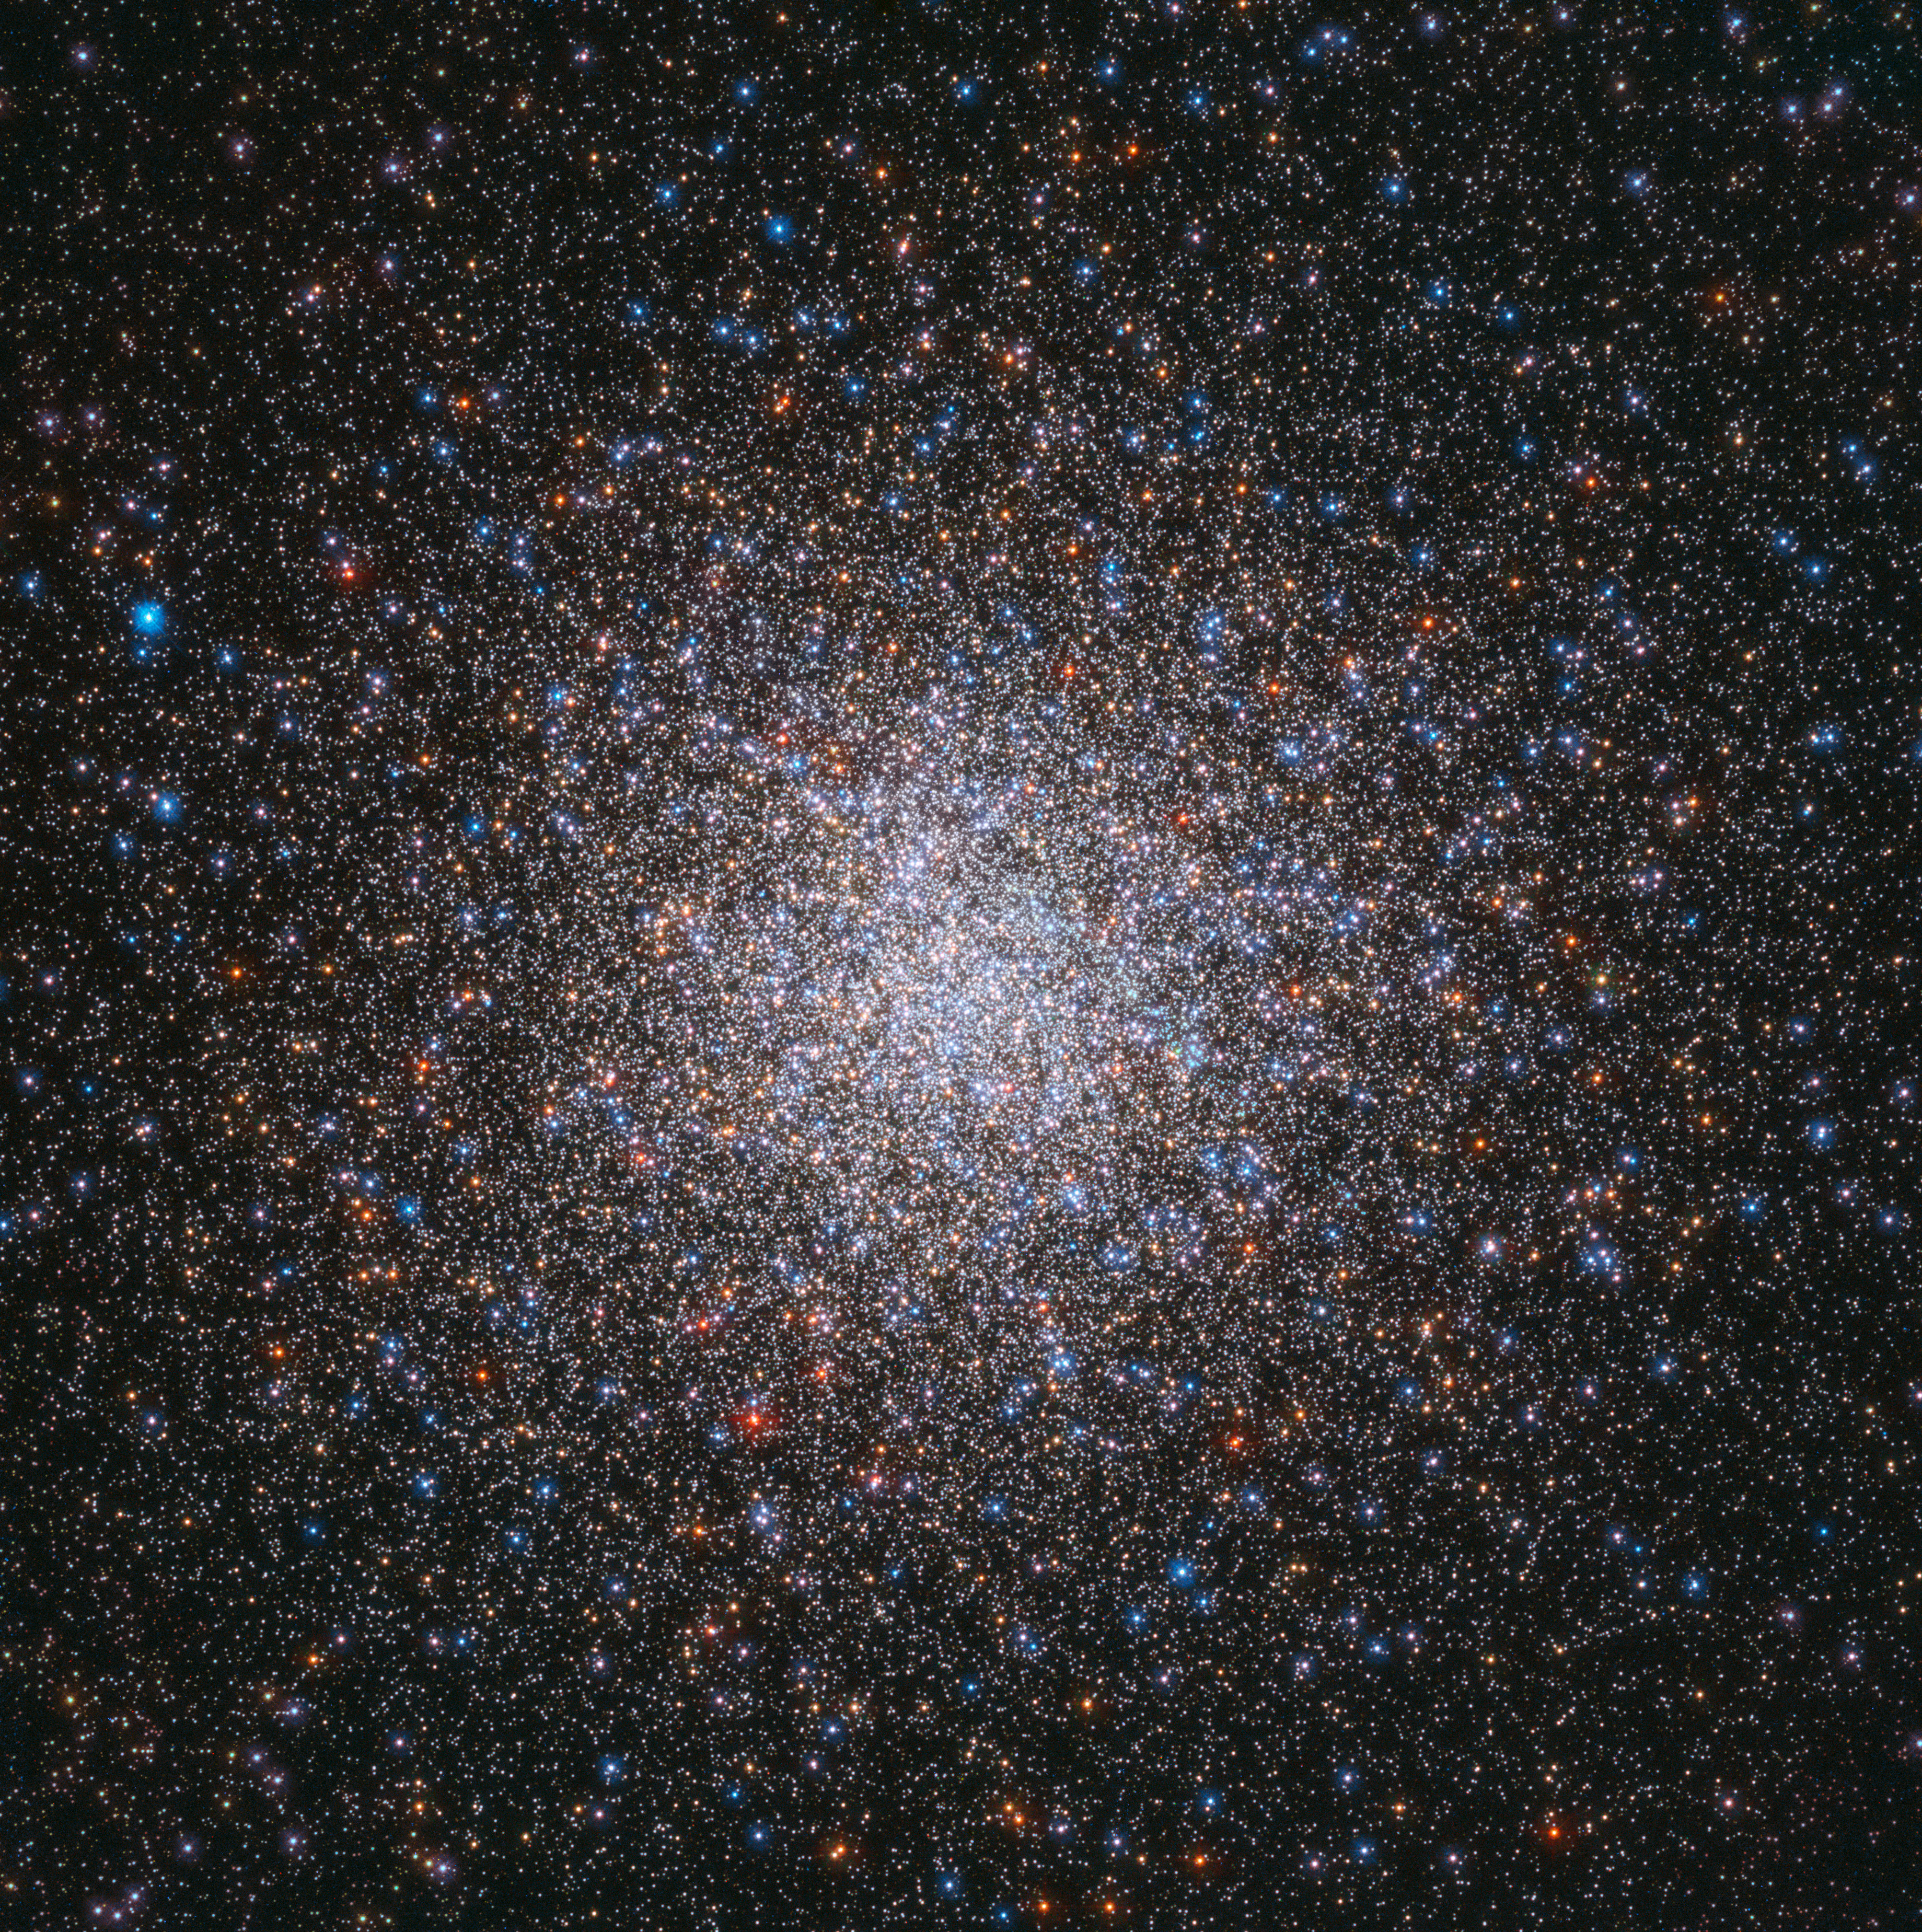
\includegraphics[width=\textwidth]{placeholder-m2.jpg}
            \caption*{The globular cluster M2}
        \end{figure}
    \end{columns}
\end{frame}

\begin{frame}{M2's Mass Density Profile}
    \begin{itemize}
        \item Characterized by a \alert{highly concentrated core}.
        \item High central density, with a very steep profile.
        \item Well-modeled by standard globular cluster profiles (e.g., King or Wilson models).
        \item High gravitational binding results in a very stable, spherically symmetric profile.
    \end{itemize}
    \begin{figure}
        \centering
        % Placeholder for a graph of M2's density profile
        %\includegraphics[width=0.7\textwidth]{placeholder-m2-profile.png}
        %\caption{Graph showing a steep, centrally peaked density profile for M2.}
    \end{figure}
\end{frame}

\section{The Open Cluster M34}

\begin{frame}{Case Study: M34}
    \begin{columns}[c]
        \column{.5\textwidth}
        \begin{itemize}
            \item Located in the constellation Perseus.
            \item Intermediate age, around \num{200} million years.
            \item Smaller and less populous, with \num{100} to \num{400} members.
        \end{itemize}
        \column{.5\textwidth}
        \begin{figure}
        \centering
            \includegraphics[width=\textwidth]{m34_rp_banzai.png}
            \caption*{The open cluster M34}
        \end{figure}
    \end{columns}
\end{frame}

\begin{frame}{M34's Mass Density Profile}
    \begin{itemize}
        \item Much \alert{lower overall stellar density} compared to M2.
        \item Less concentrated core and a much shallower profile.
        \item Not as symmetrical, reflecting its "fluffier" and less bound nature.
        \item Susceptible to tidal forces from the Milky Way, leading to its eventual dispersion.
    \end{itemize}
    \begin{figure}
        \centering
        % Placeholder for a graph of M34's density profile
        %\includegraphics[width=0.7\textwidth]{placeholder-m34-profile.png}
        %\caption{Graph showing a shallower, less peaked density profile for M34.}
    \end{figure}
\end{frame}

\section{Comparison and Conclusion}

\begin{frame}{M2 vs. M34: A Direct Comparison}
    \begin{table}
        \centering
        \begin{tabular}{l l l}
            \toprule
            \textbf{Feature} & \textbf{Globular Cluster M2} & \textbf{Open Cluster M34} \\
            \midrule
            Age & $\sim$\num{13} billion years & $\sim$\num{200} million years \\
            Population & $>150,000$ stars & \num{100}--\num{400} stars \\
            Shape & Highly spherical, compact & Irregular, loosely packed \\
            Density Profile & Steep, highly peaked & Shallow, less concentrated \\
            Stability & Dynamically stable & Prone to disruption \\
            \bottomrule
        \end{tabular}
        \caption{Comparison of key features for M2 and M34.}
    \end{table}
\end{frame}

\begin{frame}{S/N Calculations}
    \begin{table}
        \centering
        \begin{tabular}{l l l l l l l}
            \toprule
            \textbf{Object} & \textbf{Filter} & \textbf{Mag} & \textbf{\# Exp} & \textbf{Int t} & \textbf{S/N} & \textbf{S/N stack}\\
            \midrule
            M2 & SDSS g' & 14 & 3 & 8 & 180–300 & 310–520\\
            M2 & SDSS g' & 18 & 3 & 120 & 45–60 & 78–104\\
            M2 & SDSS g' & 21.5 & 3 & 300 & 20–24 & 35–42\\
            M34 & SDSS g' & 11 & 3 & 10 & 200–300 & 350–520\\
            M34 & SDSS g' & 17.5 & 3 & 60 & 60–80 & 104–139\\
            M34 & SDSS g' & 19 & 3 & 180 & 25–30 & 43–52\\
            M2 & SDSS r' & 14 & 3 & 8 & 250–400 & 430–690\\
            M2 & SDSS r' & 18 & 3 & 90 & 50–70 & 87–121\\
            M2 & SDSS r' & 20.5 & 3 & 240 & 22–28 & 38–49\\
            M34 & SDSS r' & 11 & 3 & 10 & $>$ 300& $\gg$ 500\\
            M34 & SDSS r' & 17.5 & 3 & 60 & $70–90$ & 120–155\\
            M34 & SDSS r' & 19 & 3 & 180 & 30–35 & 52–61\\
            \bottomrule
        \end{tabular}
        \caption{S/N calculations for each filter}
    \end{table}
\end{frame}

\begin{frame}{Image stacking to increase S/N ratio}
    Each exposure contains the same signal (star light) but different noise (random variations).
    
    Adding or averaging multiple exposures reinforces the signal and averages down the noise.

    \begin{equation*}
        S/N_{stacked}=S/N_{single} × \sqrt{N}
    \end{equation*}

    Where $N$ is the number of images. 

    This allows shorter individual exposures (avoids saturation) and improves photometric precision and faint-star detection.

\end{frame}



\begin{frame}[fragile]
    \frametitle{References}
    \footnotesize
    % Assuming a reference.bib file exists in the same directory
    \bibliography{reference.bib}
    \bibliographystyle{apalike}
\end{frame}

\begin{frame}
    \Huge{\centerline{\textbf{Thank You}}}
\end{frame}

%----------------------------------------------------------------------------------------

\end{document}
